% !TeX program = pdflatex
% !BIB program = bibtex
% Template LaTeX file for DAFx-19 papers
%
% To generate the correct references using BibTeX, run
%     latex, bibtex, latex, latex
% modified...
% - from DAFx-00 to DAFx-02 by Florian Keiler, 2002-07-08
% - from DAFx-02 to DAFx-03 by Gianpaolo Evangelista
% - from DAFx-05 to DAFx-06 by Vincent Verfaille, 2006-02-05
% - from DAFx-06 to DAFx-07 by Vincent Verfaille, 2007-01-05
%                          and Sylvain Marchand, 2007-01-31
% - from DAFx-07 to DAFx-08 by Henri Penttinen, 2007-12-12
%                          and Jyri Pakarinen 2008-01-28
% - from DAFx-08 to DAFx-09 by Giorgio Prandi, Fabio Antonacci 2008-10-03
% - from DAFx-09 to DAFx-10 by Hannes Pomberger 2010-02-01
% - from DAFx-10 to DAFx-12 by Jez Wells 2011
% - from DAFx-12 to DAFx-14 by Sascha Disch 2013
% - from DAFx-15 to DAFx-16 by Pavel Rajmic 2015
% - from DAFx-16 to DAFx-17 by Brian Hamilton 2016
% - from DAFx-18 to DAFx-19 by Dave Moffat 2019
%
% Template with hyper-references (links) active after conversion to pdf
% (with the distiller) or if compiled with pdflatex.
%
% 20060205: added package 'hypcap' to correct hyperlinks to figures and tables
%                      use of \papertitle and \paperauthorA, etc for same title in PDF and Metadata
%
% 1) Please compile using latex or pdflatex.
% 2) If using pdflatex, you need your figures in a file format other than eps! e.g. png or jpg is working
% 3) Please use "paperftitle" and "pdfauthor" definitions below

%------------------------------------------------------------------------------------------
%  !  !  !  !  !  !  !  !  !  !  !  ! user defined variables  !  !  !  !  !  !  !  !  !  !  !  !  !  !
% Please use these commands to define title and author(s) of the paper:
\def\papertitle{Real-time Physical Model for Analog Tape Machines}
\def\paperauthorA{Jatin Chowdhury}

% Authors' affiliations have to be set below

%------------------------------------------------------------------------------------------
\documentclass[twoside,a4paper]{article}
\usepackage{dafx_19}
\usepackage{amsmath,amssymb,amsfonts,amsthm}
\usepackage{euscript}
\usepackage[latin1]{inputenc}
\usepackage[T1]{fontenc}
\usepackage{ifpdf}

\usepackage[english]{babel}
\usepackage{caption}
\usepackage{subfig} % or can use subcaption package
\usepackage{color}

\setcounter{page}{1}
\ninept

\usepackage{times}
% Saves a lot of ouptut space in PDF... after conversion with the distiller
% Delete if you cannot get PS fonts working on your system.

% pdf-tex settings: detect automatically if run by latex or pdflatex
\newif\ifpdf
\ifx\pdfoutput\relax
\else
   \ifcase\pdfoutput
      \pdffalse
   \else
      \pdftrue
\fi

\ifpdf % compiling with pdflatex
  \usepackage[pdftex,
    pdftitle={\papertitle},
    pdfauthor={\paperauthorA},
    colorlinks=false, % links are activated as colror boxes instead of color text
    bookmarksnumbered, % use section numbers with bookmarks
    pdfstartview=XYZ % start with zoom=100% instead of full screen; especially useful if working with a big screen :-)
  ]{hyperref}
  \pdfcompresslevel=9
  \usepackage[pdftex]{graphicx}
  \usepackage[figure,table]{hypcap}
\else % compiling with latex
  \usepackage[dvips]{epsfig,graphicx}
  \usepackage[dvips,
    colorlinks=false, % no color links
    bookmarksnumbered, % use section numbers with bookmarks
    pdfstartview=XYZ % start with zoom=100% instead of full screen
  ]{hyperref}
  % hyperrefs are active in the pdf file after conversion
  \usepackage[figure,table]{hypcap}
\fi
\usepackage{cleveref}

\title{\papertitle}

\affiliation{
\paperauthorA \,}
{\href{http://ccrma.stanford.edu}{Center for Computer Research in Music and Acoustics} \\ Stanford University \\ Palo Alto, CA \\ {\tt \href{mailto:jatin@ccrma.stanford.edu}{jatin@ccrma.stanford.edu}}}

\begin{document}
% more pdf-tex settings:
\ifpdf % used graphic file format for pdflatex
  \DeclareGraphicsExtensions{.png,.jpg,.pdf}
\else  % used graphic file format for latex
  \DeclareGraphicsExtensions{.eps}
\fi

\maketitle

\section{Abstract}
For decades, analog magnetic tape recording was the most popular
method for recording music, but has been replaced over the past 30 years first by
DAT tape, then by DAWs and audio interfaces \cite{Kadis}. Despite being replaced
by higher quality technology, many have sought to recreate a "tape" sound
through digital effects, despite the distortion, tape "hiss", and other
oddities analog tape produced. The following paper describes the general process
of creating a physical model of an analog tape machine starting from basic
physical principles, then discusses in-depth a real-time implementation
of a physical model of a Sony TC-260 tape machine.
\newline\newline
"Whatever you now find weird, ugly, uncomfortable, and nasty
about a new medium will surely become its signature. CD distortion, the jitteriness
of digital video, the crap sound of 8-bit - all of these will be cherished
and emulated as soon as they can be avoided." -Brian Eno \cite{Eno}.

\section{Continuous Time System}
Audio recorded to and played back from a tape machine can be thought of as going
through three distinct processors: the record head, tape magnetisation, and the play
head.

\subsection{The Record Head}
For an instantaneous input current $I(t)$, the magnetic field output of the record 
head is given as a function of distance along the tape ($x$), and depth into 
the tape ($y$). Using the Karlqvist medium field approximation, we find
\cite{1994tmr..book.....B}:

\begin{multline}
    H_x(x,y) = \frac{1}{\pi} H_0 \Big(\tan^{-1} \Big(\frac{(g/2) + x}{y} \Big) \\
    + \tan^{-1} \Big(\frac{(g/2) - x}{y} \Big) \Big)
    \label{eq1}
\end{multline}
\begin{equation}
    H_y(x,y) = \frac{1}{2 \pi} H_0 \ln \Big(\frac{((g/2) - x)^2 + y^2}{((g/2) + x)^2 + y^2} \Big)
    \label{eq2}
\end{equation}
%
where $g$ is the head gap, and $H_0$ is the deep gap field, given by:

\begin{equation}
    H_0 = \frac{NEI}{g}
\end{equation}
%
where $N$ is the number of turns coils of wire around the head, and $E$ is the head 
efficiency which can be calculated by:

\begin{equation}
    E = \frac{1}{1 + \frac{l  A_g}{\mu_r g} \int_{core} \frac {d \vec{l}}{A(l)}}
\end{equation}
%
where $A_g$ is the gap area, $\mu_r$ is the core permeability relative to 
free space ($\mu_0$), and $A(l)$ is the cross-sectional 
area of the core as a function of length.

\subsection{Tape Magnetisation}
The magnetic field being recorded to tape can be described using 
a hysteresis loop, as follows \cite{1994tmr..book.....B}:

\begin{equation}
    \vec{M}(x,y) = F_{Loop}(\vec{H}(x,y))
\end{equation}
%
where $F_{Loop}$ is a generalized hysteresis function.
\newline\newline
Using the Jiles-Atherton magnetisation model, the following
differential equation describes magnetisation ($M$) as a function 
of magnetic field ($H$) \cite{Hysteresis}:

\begin{equation}
    \frac{dM}{dH} = \frac{(1-c) \delta_M (M_{an} - M)}{(1-c) \delta k - \alpha (M_{an} - M)} + c \frac{dM_{an}}{dH}
    \label{eq5}
\end{equation}
%
where $c$ is the ratio of normal and anhysteric initial susceptibilities,
$k$ is a measure of the width of the hysteresis
loop, $\alpha$ is a mean field parameter, representing inter-domain
coupling, and $\delta$ and $\delta_M$ are given by:

\begin{equation}
    \delta = \begin{cases}
        1 & \text{if H is increasing} \\
        -1 & \text{if H is decreasing}
    \end{cases}
\end{equation}
\begin{equation}
    \delta_M = \begin{cases}
        1 & \text{if $\delta$ and $M_{an} - M$ have the same sign} \\
        0 & \text{otherwise}
    \end{cases}
\end{equation}
%
$M_{an}$ is the anisotropic magnetisation given by:

\begin{equation}
    M_{an} = M_s L \Big( \frac{H + \alpha M}{a} \Big)
\end{equation}
%
where $M_s$ is the magnetisation saturation, $a$ characterizes the shape
of the anhysteric magnetisation and $L$ is the Langevin function:

\begin{equation}
    L(x) = \coth (x) - \frac{1}{x}
\end{equation}

\subsection{Play Head}
\subsubsection{Ideal Playback Voltage}
The ideal playback voltage as a function of tape magnetisation is given by
\cite{1994tmr..book.....B}:

\begin{equation}
    V(x) =  NWEv \mu_0 \int_{-\infty}^{\infty} dx' \int_{-\delta/2}^{\delta/2} dy' \vec{h}(x' + x, y') \cdot \frac{\vec{M}(x', y')}{dx}
    \label{eq11}
\end{equation}
%
where $N$ is the number of turns of wire, $W$ is the width of the playhead, $E$ is the playhead
efficiency, $v$ is the tape speed, and $\mu_0$ is the permeability of free space.
Note that $V(x) = V(vt)$ for constant $v$. $\vec{h}(x, y)$ is defined as:

\begin{equation}
    \vec{h} (x, y) \equiv \frac{\vec{H} (x, y)}{NIE}
    \label{eq12}
\end{equation}
%
where $\vec{H} (x, y)$ can be calculated by \cref{eq1,eq2}.

\subsubsection{Loss Effects}
There are several frequency-dependent loss effects associated with playback,
described as follows \cite{Kadis}:

\begin{equation}
    V(t) = V_0(t) [e^{-kd}] \Big[\frac{1 - e^{-k \delta}}{k \delta} \Big] \Big[\frac{\sin (kg /2)}{kg/2} \Big]
    \label{eq:lossEffects}
\end{equation}
%
for sinusoidal input $V_0(t)$, where $k$ is the wave number, $d$ is the distance between the tape and the playhead,
$g$ is the gap width of the play head, and $\delta$ is the thickness of the tape. The wave number
is given by:

\begin{equation}
    k = \frac {2 \pi f}{v}
    \label{eq:wavenumber}
\end{equation}
%
where $f$ is the frequency and $v$ is the tape speed.

\section{Digitizing the System}
\subsection{Record Head}
For simplicity, let us assume,
\begin{equation}
    \vec{H}(x,y,t) = \vec{H}(0,0,t)
\end{equation}
%
In this case $H_y \equiv 0$, and $H_x \equiv H_0$. Thus,
\begin{equation}
    H(t) = \frac{NEI(t)}{g}
    \label{eq15}
\end{equation}
%
or,
\begin{equation}
    \hat{H}(n) = \frac{NE\hat{I}(n)}{g}
    \label{eq:Hin}
\end{equation}

\subsection{Hysteresis}
Beginning from \cref{eq5}, we can find the derivative of $M$ w.r.t. time,
as in \cite{Hysteresis}:
\begin{equation}
    \frac{dM}{dt} = \frac{\frac{(1-c) \delta_M (M_sL(Q) - M)}{(1-c) \delta k - \alpha (M_sL(Q) - M)} \frac{dH}{dt} + c \frac{M_s}{a} \frac{dH}{dt} L'(Q)}{1 - c \alpha \frac{M_s}{a} L'(Q)}
    \label{eq:dmdt}
\end{equation}
%
where $Q = \frac{H + \alpha M}{a}$, and

\begin{equation}
    L'(x) = \frac{1}{x^2} - \coth^2(x) + 1
\end{equation}
%
Note that \cref{eq:dmdt} can also be written in the general form for non-linear
Ordinary Differential Equations:
\begin{equation}
    \frac{dM}{dt} = f(t,M,\vec{u})
\end{equation}
where $\vec{u} = \begin{bmatrix}
    H \\
    \dot{H}
    \end{bmatrix}$.
\newline\newline
Using the trapezoidal rule for derivative approximation, we find:

\begin{equation}
    \dot{\hat{H}}(n) = 2\frac{\hat{H}(n) - \hat{H}(n-1)}{T} - \dot{\hat{H}}(n-1)
    \label{eq:hDeriv}
\end{equation}
%
We can use the Runge-Kutta 4th order method \cite{Yeh} to find an explicit solution
for $\hat{M}(n)$:
\begin{align}
\begin{split}
    k_1 &= T f \Big(n-1, \hat{M}(n-1), \hat{\vec{u}}(n-1) \Big)\\
    k_2 &= T f \Big(n - \frac{1}{2}, \hat{M}(n-1) + \frac{k_1}{2}, \hat{\vec{u}}  \Big(n-\frac{1}{2} \Big) \Big)\\
    k_3 &= T f \Big(n- \frac{1}{2}, \hat{M}(n-1) + \frac{k_2}{2}, \hat{\vec{u}} \Big(n-\frac{1}{2} \Big) \Big)\\
    k_4 &= T f \Big(n, \hat{M}(n-1) + k_3, \hat{\vec{u}}(n) \Big)\\
    \hat{M}(n) &= \hat{M}(n-1) + \frac{k_1}{6} + \frac{k_2}{3} + \frac{k_3}{3} + \frac{k_4}{6}
\end{split}
\end{align}
%
We use linear interpolation to find the half-sample values used to calculate $k_2$ and $k_3$.

\subsubsection{Numerical Considerations}
To account for rounding errors in the Langevin function for values close to 
zero, we use the following approximation about zero, as in \cite{Hysteresis}:
\begin{equation}
    L(x) = \begin{cases}
        \coth(x) - \frac{1}{x} & \text{for $|x| > 10^{-4}$} \\
        \frac{x}{3} & \text{otherwise}
    \end{cases}
\end{equation}
\begin{equation}
    L'(x) = \begin{cases}
        \frac{1}{x^2} - \coth^{2}(x) + 1 & \text{for $|x| > 10^{-4}$} \\
        \frac{1}{3} & \text{otherwise}
    \end{cases}
\end{equation}

\subsubsection{Simulation}
The digitized hysteresis loop was implemented and tested offline
in \texttt{Python}, using the constants $M_s$, $a$, $\alpha$, $k$,
and $c$ from \cite{JilesAtherton1986}. For a sinusoidal input signal
with frequency 2kHz, and varying amplitude from 800 - 2000 Amperes per
meter, the following plot shows the Magnetisation output.

\begin{figure}[ht]
    \center
    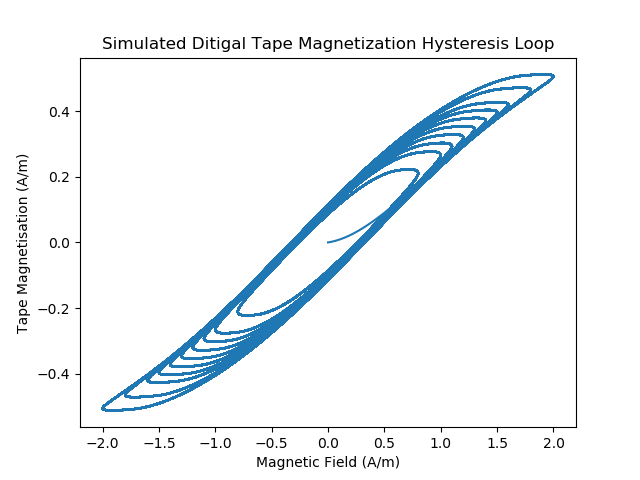
\includegraphics[width=3in]{../Simulations/Hysteresis/Sim2-M_H.png}
    \caption{\label{HysteresisSim}{\it Digitized Hysteresis Loop Simulation}}
\end{figure}
%
\subsection{Play Head}
By combining \cref{eq11} with \cref{eq12,eq15}, we get:
\begin{equation}
    V(t) =  NWEv \mu_0  g M(t)
\end{equation}
%
or,
\begin{equation}
    \hat{V}(n) =  NWEv \mu_0  g \hat{M}(n)
    \label{eq:Vout}
\end{equation}
%
\subsubsection{Loss Effects}
In the real-time system, we model the playhead
loss effects with an FIR filter, derived by
taking the inverse DFT of the
loss effects described in \cref{eq:lossEffects}.
It is worth noting that as in \cref{eq:wavenumber},
the loss effects, and therefore the FIR filter
are dependent on the tape speed.
\newline\newline
The loss effects filter was implemented and
tested offline in \texttt{Python} with tape-head 
spacing of 20 microns, head gap width of 5 microns, 
tape thickness of 35 microns, and tape speed of 15 ips.
The following plot shows the results of the simulation,
with a filter order of 100.
\begin{figure}[ht]
    \center
    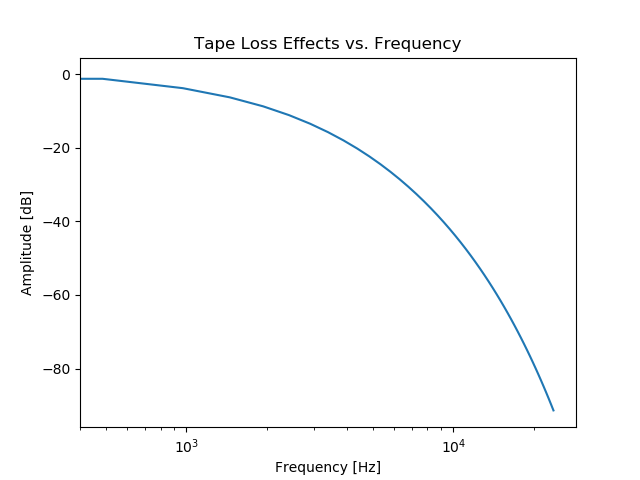
\includegraphics[width=3in]{../Simulations/LossEffects/Loss_Effects.png}
    \caption{\label{lossEffectsSim}{\it Frequency Response of Playhead Loss Effects}}
\end{figure}
%

\section{Tape and Tape Machine Parameters}
In the following sections, we describe the implementation of
a real-time model of a Sony TC-260 tape machine, while attempting
to preserve generality so that the process can be repeated for any
other similar reel-to-reel tape machine.

\subsection {Tape Parameters}
A typical reel-to-reel tape such as the Sony TC-260 uses 
Ferric Oxide ($\gamma F_2O_3$) magnetic tape. The following
properties of the tape are necessary for the tape hysteresis
process \cref{eq:dmdt}:
\begin{itemize}
\item Magnetic Saturation ($M_s$): For Ferric Oxide tape
the magnetic saturation is $3.5e5$ (A/m) \cite{jilesBook}
\item Hysteresis Loop Width ($k$): For soft materials, $k$ can be approximated
as the coercivity, $H_c$ \cite{Jiles1992}. For Ferric Oxide, $H_c$ is approximately
$27$ kA/m \cite{jilesBook}.
\item Anhysteric magnetisataion ($a$): Knowing the coercivity and remnance magnetism of Ferric Oxide
\cite{jilesBook}, we can calculate $a$ = 22  kA/m by the method described in
\cite{Jiles1992}
\item Ratio of normal and hysteris initial susceptibilities ($c$): From \cite{Jiles1992}, $c$ = 1.7e-1.
\item Mean field parameter ($\alpha$): From \cite{Jiles1992}, alpha = 1.6e-3
\end{itemize}

\subsection{Tape Machine Parameters}
\subsubsection {Record Head}
To determine the magnetic field output of the
record head using \cref{eq:Hin}, the following parameters 
are necessary:
\begin{itemize}
\item Input Current ($\hat{I} (n)$): For the Sony TC-260
the input current to the record head is approximately
0.1 mA peak-to-peak \cite{RefManual}.
\item Gap Width ($g$): The gap width for recording heads
can range from 2.5 to 12 microns \cite{Kadis}.
\item Turns of wire ($N$): The number of turns of wire
is typically on the order of 100 \cite{1994tmr..book.....B}.
\item Head Efficiency ($E$): The head efficiency is typically
on the order of 0.1 \cite{1994tmr..book.....B}.
\end{itemize}
%
These values result in a peak-to-peak magnetic field
of approximately 5e5 A/m.

\subsubsection{Play Head}
Similar to the record head, the following parameters
are needed to calculate the output voltage using
\cref{eq:Vout,eq:lossEffects} (note that values are only included
here if notably different from the record head):
\begin{itemize}
\item Gap Width ($g$): The play head gap width ranges from
1.5 to 6 microns\cite{Kadis}.
\item Head Width ($W$): For the Sony TC-260, the play head
width is 0.125 inches (note that this is the same as the
width of one track on the quarter-inch tape used by the 
machine) \cite{RefManual}.
\item Tape Speed ($v$): The Sony TC-260 can run at 3.75 inches
per second (ips), or 7.5 ips \cite{RefManual}. Note that many
 tape machines can run at 15 or 32 ips \cite{Kadis}.
\item Tape Thickness ($\delta$): Typical tape that would be used
with the TC-260 is on the order of 35 microns thick \cite{RefManual}.
\item Spacing ($d$): The spacing between the tape and the play
head is highly variable between tape machines. For a typical
tape machine spacing can be as high as 20 microns \cite{Kadis}.
\end{itemize}

\subsection{Tape Bias}
A typical analog recorder adds a high-frequency "bias"
current to the signal to avoid the "deadzone" effect when the input signal
crosses zero, as well as to linearize the output. The input
current to the record head can be given by
\cite{Camras:1987:MRH:27189}:
\begin{equation}
    \hat{I}_{head}(n) = \hat{I}_{in}(n) + B \cos(2 \pi f_{bias} n T)
\end{equation}
%
Where the amplitude of the bias current $B$ is usually
about one order of magnitude larger than the input,
and the bias frequency $f_{bias}$ is well above the
audible range. The plot below shows a unit-amplitude,
2 kHz sine wave biased by a 50 kHz sine wave with amplitude 5.
To recover the correct output signal, tape machines use a
lowpass filter, with a cutoff frequency well below the bias
frequency, thought still above the audible range \cite{Kadis}.
\begin{figure}[ht]
    \center
    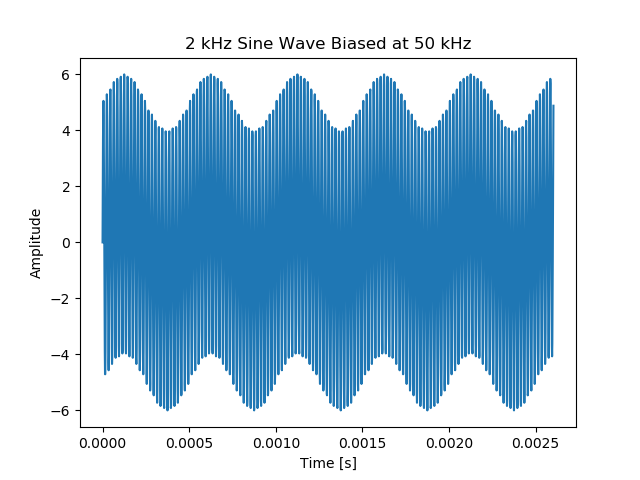
\includegraphics[width=3in]{../Simulations/Bias/BiasEx.png}
    \caption{\label{Bias}{\it Example of a biased signal}}
\end{figure}
\newline\newline
For the Sony TC-260, the bias frequency is 55 kHz, with a gain
of 5 relative to the input signal. The lowpass filter used to recover
the audible signal has a cutoff at 24 kHz, though note that due to
the frequency response of the playhead loss effects, the effects
of this filter may be essentially neglible to the real time system.
\cite{RefManual}

\subsection{Wow and Flutter}
Each tape machine has characteristic timing imperfections
known as ``wow'' and/or ``flutter.'' These imperfections
are caused by minor changes in speed from the motors
driving the tape reels, and can cause fluctuations in
the pitch of the output signal. To characterize these
timing imperfections, we use a method similar to \cite{tapeDelay}:
We recorded a pulse train of 1000 pulses through a TC-260,
then recorded the pulses back from the tape. \Cref{timingSim}
below shows a section of a superimposed plot of the original
pulse train against the pulse train recorded from the tape
machine. From this data, we were able to generate a periodic
function that accurately models the timing imperfections of
the TC-260. The process was performed at both 7.5 ips and 3.75
ips. In the real-time system, the timing imperfection model
is used to inform a modulating delay line, to achieve the
signature "wow" effect of an analog tape machine.

\begin{figure}[ht]
    \center
    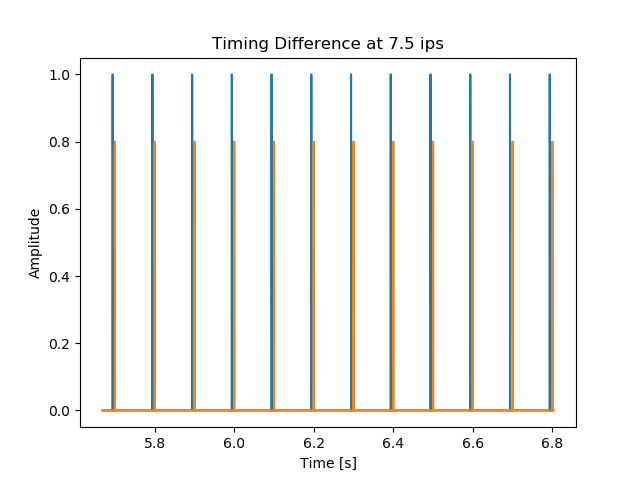
\includegraphics[width=3in]{../Simulations/TimingEffects/timing_diff_7-5.png}
    \caption{\label{timingSim}{\it Input pulse train superimposed with pulse train recorded from TC-260}}
\end{figure}
%

\section{Real-Time Implementation}
@TODO
\subsection{Oversampling} %@TODO; move this section somewhere else
If no oversampling is used, the system will be unstable
for input signal at the Nyquist frequency, due to limitations
of the trapezoid rule derivate approximation used in \cref{eq:hDeriv}.
To avoid this, a lowpass filter with cutoff frequency below Nyquist
should suffice. However, due to aliasing caused by the nonlinearity
of the tape hysteresis model, oversampling is necessary to mitigate
aliasing artifacts \cite{Yeh}. Further, the system must be able to
faithfully recreate not only the frequencies in the audible range
but the bias frequencies as well. Since the minimum standard audio sampling
rate is 44.1 kHz, and the minimum standard biasing frequency is approximately
50 kHz \cite{Camras:1987:MRH:27189}, a minimum oversampling factor of 3x is
required. In the real-time implementation, we use a minimum
oversampling factor of 4x, with options to oversample at 8x or 16x
if the user desires.

%\newpage
\nocite{*}
\bibliographystyle{IEEEbib}
\bibliography{references}

\end{document}
